
\chapter{\label{cha: Graph Transformation Approach }Graph Transformation Approach}

\section{ Introduction }
i will show in this chapter my work which is Optimise Multi Agent system  
represented in OMACS Framework , but the problem is OMACS does not have any 
Any algorithm to do that 

Because of That i represent the second Frameword PNS which contain an Algorithm 
to find the optimum structure .

so we need to work on th Transformation from OMACS MODEL into PNS MODEL



 
\section{model and Meta-Model }
What is Metamodeling 

Meta \quad means literally After in Greek.
n Computer Science, the term is used heavily and with
several different meanings : 
\begin{enumerate}
\item In Databases, metadata means  data about data  and
		refer to data dictionaries, repositories, etc.
\item In Programming Languages, metainterpreter is an
		interpreter of a (program) interpreter
\item In Conceptual Modeling, metamodel is a model of a
		data model, e.g., an E-R model of the relational model,
		or an ER model of the ER model.
		
\end{enumerate}
 
Data is modelled by metadata (schemas,  classes,...)
which are parts of the metamodel; these units are
instances of meta 2 data which are parts of a
metametamodel
[from:REF/other/Meta]



Meta-Modelling, which is the process of modelling formalisms. 

Formalisms are described as models described in meta-formalisms. 

The latter are nothing  
but expressive enough formalisms, such as Entity Re-
lationship diagrams (ER) or UML class diagrams.

A model of a meta-formalism is called a meta-meta-
model; a model of a formalism is called a meta-model.
[from:REF//other/Meta-modelling and graph grammars for multi-paradigm modelling in AToM 3]

\subsection{Architercteur of Meta-Modeling}
The traditional meta-model architecture proposed by OMG is based on 4 Levels
described in this Figure \ref{fig:Pyramid of Meta-Level} .

\begin{enumerate}
\item \textbf{Model} is a simplified abstraction of a studied system, constructed in a
Particular intent. 

It should be able to be used to answer questions about the system

A system is a theoretical construct formed by the mind on a subject
Example, an idea that is implemented to explain a physical phenomenon that can
be represented by a mathematical model) 

\item \textbf{Meta Model} is a language that expresses models. It defines
Concepts as well as the relations between concepts necessary for the expression of models . 
A model is a possible construction of the metamodel in which it is defined.

In the Literature, a model is said to conform to the metamodel in which it is defined

\item \textbf{Meta Meta Model} is a language used to express metamodels. 
For Ability to interpret a meta-model requires a description of the language in which
It is written: a meta-model for meta-models. 
It is, of course, Meta-model by the term meta-meta-model  . 

To limit the  Number of levels of abstraction, the meta-meta-model 
must have the ability to describe itself, even. 
 

\end{enumerate}

MOF : (Meta-Object Facility) is set of Interfaces allow to define 
the syntax and semantic of modilisation language , is devloped by OMG

\begin{figure}[th]
	\centering
		\includegraphics{Chapiter3/img/Pyramid}
	\caption{\label{fig:Pyramid of Meta-Level}Pyramid of Meta-Level}
\end{figure} 



\section{Transformation Model}


\subsection{Definition}
A transformation is the automatic generation of a target model from a
Source model, according to a transformation definition. 

A definition of transformation Is a set of transformation rules 
that describes how a source model
Can be transformed into a target model

 the transformation of the model is
For mapping models across domains to analyze or
The automatic generation of code from themselves

\section{Norme of Transformation } 
 The process of graph transformation consists in the iterative application of
Rule to a graph.

 Each rule application replaces a part of the graph by a
As defined in the rule. 

The mechanics of the graph transformation
Works as follows: 
\begin{enumerate}
\item select an applicable rule from the set of rules;
\item Apply this rule to the input graph;

\item Search for another applicable rule  
\item do these steps Until  no rule can be applied

\end{enumerate}

 
This operation is based on a
A set of rules respecting a particular syntax, called the grammar model of
Graph

before starting apply rules we execute initial action , 
its prepare the envirenement to apply these rules
and ending with Final Action , it about cleaning the after these rules

\begin{figure}[th]
	\centering
		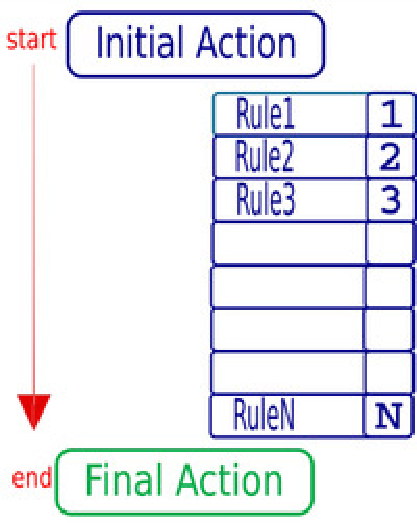
\includegraphics[scale=0.8]{Chapiter3/img/gt}
	\caption{\label{fig:Cycle of Tranformation}Cycle of Transformation}
\end{figure} 

 
\section{Graph Grammar} 
Every Graph Grammer contain a set of rules  to use in graph transformation
and its define by :
R = (LHS, RHS, K, glue, emb, cond). 
\begin{itemize}
 
\item LHS graph of left part.
\item RHS gra5ph of right part.
\item A subgraph K of LHS.
\item A glue occurrence of K in RHS that connects the subgraph with the part graph  right.
\item An embedding relation emb which connects the vertices of the graph on the left-hand side
And those of the graph on the right-hand side.
\item A set cond which indicates the conditions of application of the rule
\end{itemize}

Applying a rule R = (LHS, RHS, K, glue, emb, cond) to a graph G produced in
Result a graph H according to the following five steps

\begin{figure}[th]
	\centering
		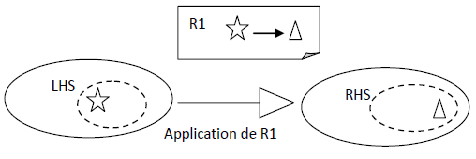
\includegraphics{Chapiter3/img/r}
	\caption{\label{fig:Rule Application}Rule Application}
\end{figure} 

\begin{enumerate}
\item  Choose an instance of the left-hand LHS graph in G.
\item Check the conditions of application according to Cond.
\item Remove the occurrence of LHS (up to K) from G and the hanging arcs (all
Arcs having lost their sources and / or their destinations). This provides the graph of
Context D of LHS which left an occurrence of K
\item
Paste the context graph D and the RHS right-hand graph according to the occurrence
Of K in k = 1, .., $\infty$ D and in RHS, it is the construction of the union of disjunction
Of D and RHS, and for each point in K, identify the corresponding point in
D with the corresponding point in RHS
\item
Press the right-hand graph in the LHS context graph following the
Embedding relation emb: for each incident arc removed with a vertex v in
D and with a vertex v1 in the occurrence of LHS in G, and for each vertex
V2 in RHS, a new incident arc is established (same label) with the image of v
And the vertex v2 provided that (v1 , v2 ) belongs to emb. 
\end{enumerate}


 
\section{ Transformation system } 

We define a graph transformation system as a rewriting system
Of graph that applies the rules of the graph grammar on its initial graph of
Iteratively by the Engine , until no more rules are applicable

\begin{enumerate}
\item Define the  source and target Meta-Model 
\item Create the the source model according to the source Meta-Model 
\item Define transformation rules to Transform from source model into target model 
\end{enumerate}
\vspace{1cm}
Finally the engine read source model and apply the transformation rules and write target model
as the following Figure \ref{fig:Transformation System}
\vspace{1cm} 

\begin{figure}[th]
	\centering
		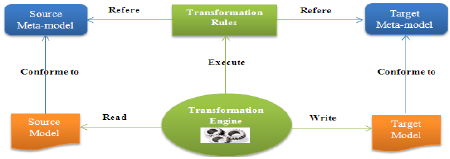
\includegraphics{Chapiter3/img/sys}
	\caption{\label{fig:Transformation System}Transformation System}
\end{figure} 
 
\pagebreak

\section{AToM $^{3}$}

AToM$^{3}$ (A Tool for Multi-formalism and Meta-Modeling) is a tool for model-
Multi-paradigm model developed in the MSDL (Modeling, Simulation and
Design Lab) of the Computer Science Institute at McGill University Montreal, Canada.

It is Developed with the Python language in collaboration with Professor Juan de Lara de
The Autonomous University of Madrid (UAM), Spain  
AToM3 is developed to satisfy two main features that are 
\begin{enumerate}
\item Meta-modeling 
\item The transformation of models
\end{enumerate}

The formalisms and models in AToM3 are described graphically. 
From a Meta-specification (example: in the Entity-relation formalism) of a formalism, AToM3
Generates a tool to visually manipulate (create and modify) the models described in
The specified formalism.

 The transformations of the models are realized by the rewriting
Graphs, which can be expressed in a declarative way as a model of
Grammar of graphs

 figure \ref{fig:AToM3 Window} illustrates the interface of AToM3 

\begin{figure}[th]
	\centering
		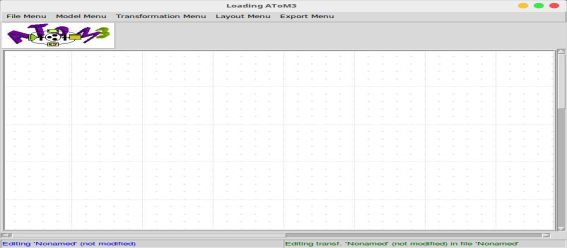
\includegraphics{Chapiter3/img/atom3}
	\caption{\label{fig:AToM3 Window}AToM $^{3}$ Window}
\end{figure} 
\subsection{Classes in AToM$^{3}$ }
In this work we use ClassDiagramm Formalism to create  our Formalism 
or Meta-Model is built in the tool so we can load it and use  it
 
In AToM$^{3}$ the meta-models can be constructed from Classes and
Relationships.

The description of classes and association relations consists of

\begin{itemize}
\item  Name
\item  Attributes
\item  Constraints
\item  Action
\item  Cardinalities
\item  Appearance
\end{itemize}

\begin{figure}[th]
	\centering
		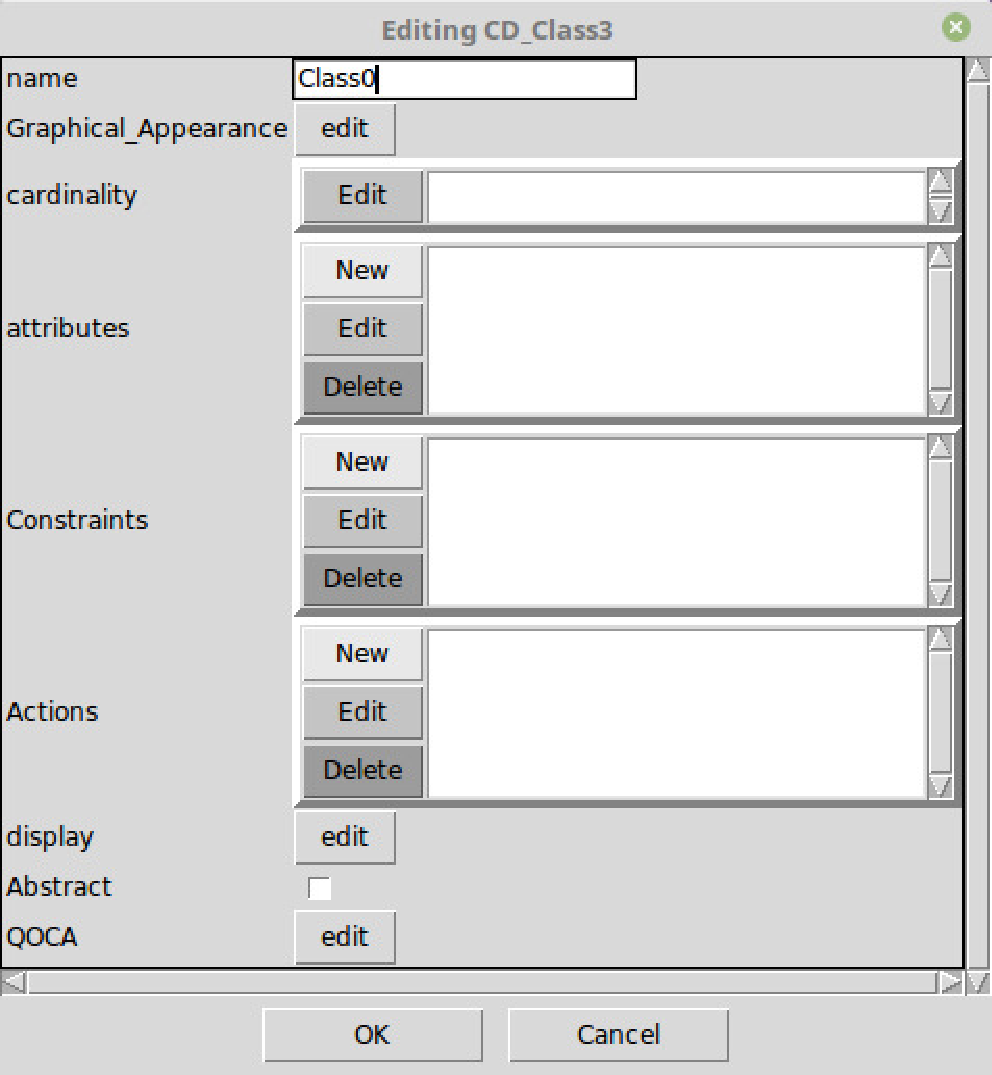
\includegraphics[scale=0.5]{Chapiter3/img/class}
	\caption{\label{fig:Class Editor}Class Editor}
\end{figure} 
\subsubsection{ Constraint }

Constraints can be specified as OCL (Constraint Object Language) or Python
They have the following properties: 
\begin{itemize}
\item  constraint name
\item  triggering event  like Drag , Move , Select ..
and launch this event before (pre-condition) or after (post-condition)
 
\end{itemize}
 

\begin{figure}[th]
	\centering
	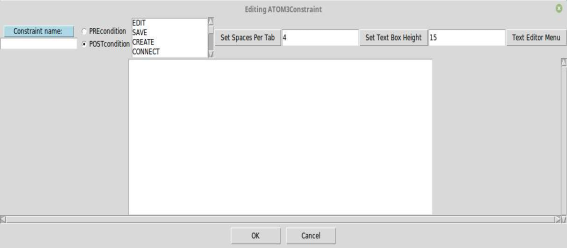
\includegraphics{Chapiter3/img/cont}
	\caption{\label{fig:Constraint Editor}Constraint Editor}
\end{figure} 
\pagebreak
\subsubsection{ Action }

An action is similar to a constraint except that it has other effects and is a
Code in Pyton only

They have the following properties :
\begin{itemize}
\item action name
\item triggering event: It can be either
	\begin{enumerate}
	\item Semantics such as saving a model
	\item Graphic or structural, such as moving or selecting an entity.
	\end{enumerate}
	
\item The execution is either
	\begin{enumerate}
	\item Before the event (precondition)
	\item  After (pots-condition) 
	\end{enumerate}

\end{itemize}
its have the same windows \ref{fig:Constraint Editor}  


\section{ Graph Grammer in AToM $^{3}$ }
In AToM3, grammar is a model characterized by
\begin{itemize}
\item An initial action.
\item A final action.
\item The set of rules. 
\end{itemize}
and this figure \ref{fig:Graph Grammar Window} Graph Grammar Editor
 
\begin{figure}[th]
	\centering 
	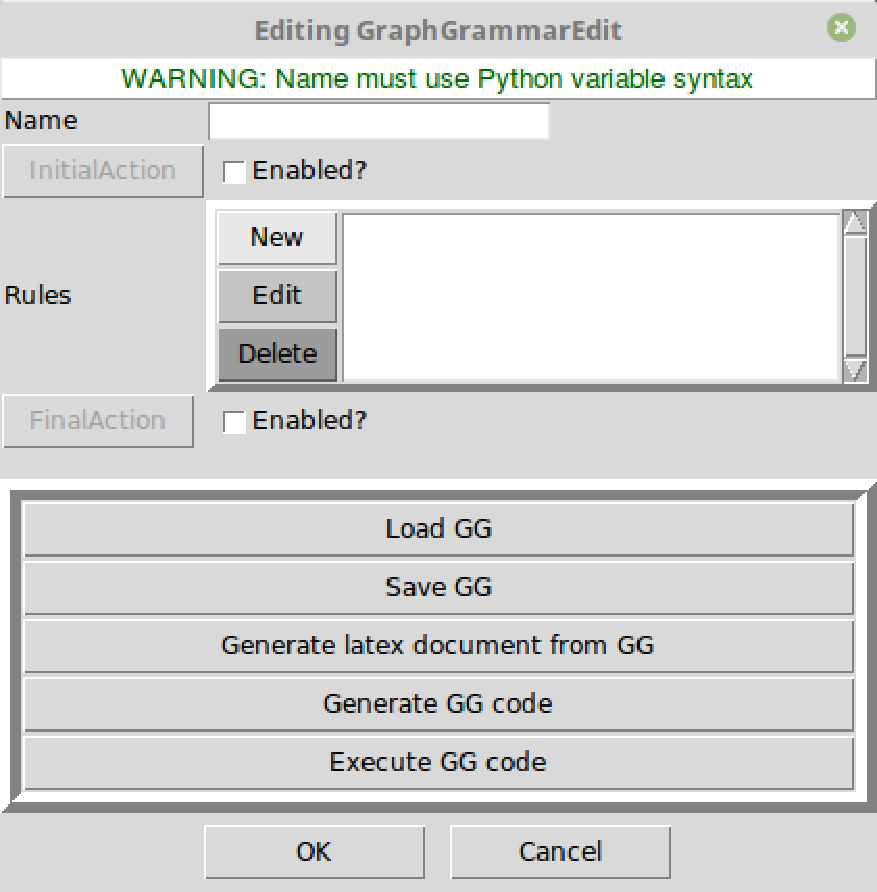
\includegraphics[scale=0.5]{Chapiter3/img/gg}
	\caption{\label{fig:Graph Grammar Window}Graph Grammar Window}
\end{figure} 
 

 Each rule consists of: 
\begin{itemize}
\item  A specific name for the rule.
\item  A priority indicating the order in which the rule is applied.
\item  A Left Hand Side (LHS) which is a graph.
\item  A right hand side (RHS) that can be a graph.
\item  A condition (Pyton code) that must be checked before the rule is
Applied.
\item An action (a Pyton code) that must be executed after the rule is
Applied
\end{itemize}


The rule editor figure \ref{fig:Rule Editor} allows the editing of the different parts of the rule as well as
The condition and action of each rule 
 
 The condition editor and the action editor of a rule are similar to the editor of
Constraints presented in Figure \ref{fig:Constraint Editor}


\begin{figure}[th]
	\centering
 	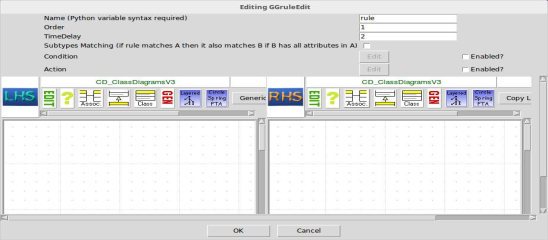
\includegraphics{Chapiter3/img/rule}
	\caption{\label{fig:Rule Editor}Rule Editor}
\end{figure} 
 


 

\section{Implementation of the Transformation (OMACS into PNS)\label{sec:OMACS into PNS} }% Our Work
To Transform OMACS Model into PNS Model should we start to :
\begin{enumerate}
\item Define OMACS Meta-Model 
\item Define PNS Meta-Model
\item Define the rules of Transformation
\end{enumerate}


\subsection{ Meta-Model of OMACS  and PNS } 
Before start create our Meta-Model should load the Class Diagramm ToolBar ,
in OMACS Meta-Model contain set of classes :

\begin{itemize}

\item Agent  
\item Capabilities
\item Role
\item Goal

\end{itemize}
 
\begin{figure}[th]
		\centering
 	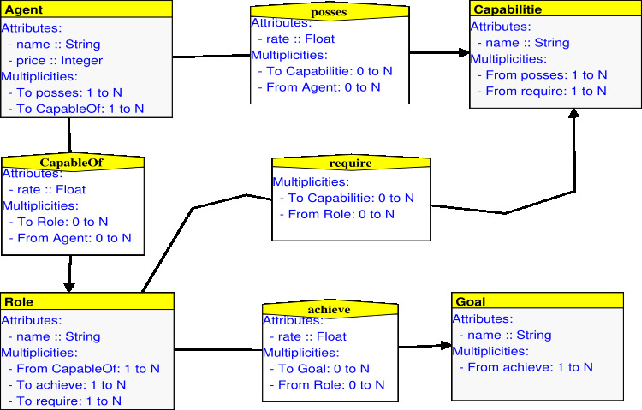
\includegraphics[scale=1.3]{Chapiter3/img/omacs}
	\caption{\label{fig:OMACS Meta-Model}OMACS Meta-Model}
\end{figure} 
 
figure \ref{fig:OMACS Meta-Model} illustrate OMACS Meta-Model  contain 4 classes 
and 4 relation   
the Attribute Name in the classes represent the name of current node ,
and the rate attribute in the relation represent  the percentage between two node .

For example between an Agent and Capabilities its means how mush this Agent possese this capibilites
 

the Same Steps should load the Class Diagramm first to create PNS Meta-Model , and its contain 4 classes and Relation
represent  : 
\begin{itemize}
	\item Raw Material  
	\item Intermediare Material
	\item Final Product
	\item Operating Unit
\end{itemize}

\begin{figure}[th] 

	\centering
 	\includegraphics[scale=0.8]{Chapiter3/img/a}
	\caption{\label{fig:PNS Meta-Model}PNS Meta-Model}
	
\end{figure} 

all material in figure \ref{fig:PNS Meta-Model} containt the same Attribute
\begin{itemize}


\item \textit{Name} : name of Material 
\item \textit{Price} : Price of Material
\item \textit{ReqFlow} : Requirment Flow means how much you have from this material in this system
\item \textit{MaxFlow} : Maximum Flow means how much your system can handle

\end{itemize}



and for the Operating Unit contain 3 Attribute : 
\begin{itemize}

\item Name : name of this Task 
\item Operating Cost Fix  : cost for entire period ,  Example for Entire year
\item Operating Cost Propotinal  :  cost for every Operating from this unit

\end{itemize}
 


\subsection{ Model in OMACS and PNS }

Starting from this  \ref{fig:OMACS Meta-Model} Meta-Model , $AToM^3$ generate a ToolBar of OMACS  , this toolbar allow us to create our OMACS Model (Multi Agent System) .
\vspace{0.1cm}
\begin{figure}[th]
	\centering
 	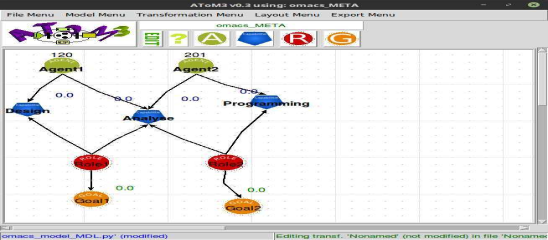
\includegraphics{Chapiter3/img/omacsMDL}
	\caption{\label{fig:OMACS Model}ToolBar for OMACS Generated by $AToM^3$ }
\end{figure} 

Example in this figure \ref{fig:OMACS Model} represent a Multi Agent system which is  a component of 2 agent and 3 Capabilities , 2 Roles , 2 Goals
\vspace{0.1cm}


its Also the same  , $AToM^3$ generate a ToolBar of PNS , load it and use it like this \ref{fig:PNS Model}

\begin{figure}[th]
	\centering
 	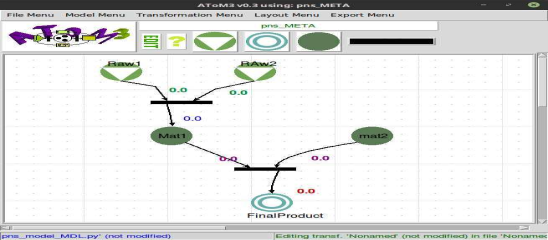
\includegraphics{Chapiter3/img/pnsMDL}
	\caption{\label{fig:PNS Model}ToolBar for PNS Generated by $AToM^3$}
\end{figure} 

represent system de production contain 2 raw material and 2 intermediate material , final product
and 2 operating unit 





\pagebreak
\subsection{ Rule of Transformation }
A grammar of graphs is a grammar consisting of a set of rules, per-
Transforming formalisms of the same nature or of a different nature. 

Each Rule is composed of two parts, the left part (LHS) and the right part (RHS).
Each part can be a subgraph of the formalisms considered in the transformation

in our work, the formalisms considered in the transformation are formalism
OMACS as source graph to be transformed into PNS a transformation target graph.
This grammar is defined using the AToM3 tool according to the following step

\begin{enumerate}
	\item Load OMACS and PNS meta-models
	\item Create the transformation grammar
	\item Define the rules of grammar
	\item Generate the executable file of the grammar
\end{enumerate}
 
\subsubsection{ Graph Grammar }
Our grammar is composed of :
\begin{description}

\item [{Rules :}]  

Each rule is characterized
By a name and execution priority. They are classified in 04 categories

\end{description}

\begin{enumerate}
\item Rules for Collect and create relation between some entitie
\item Rules for transforming nodes or links into materials or operating units .
\item Rules to links generated materials and operating units
\item Rules to cleaning unnecessary entities from the result 

\end{enumerate}
I summarized the transformation into the following steps  

\begin{itemize}

\item create link between the agent and role depending on the common capabilites

\item generate for every agent in OMACS Model into raw material in PNS Model
and the generated material has the same name and price 

\item generate for every goal in OMACS Model into intermediate material in PNS Model and the generated material has the same name  


\item the product in the target graph which is PNS Model represent the organization of the OMACS Model

\item create Operating unit for each direct link between the role and an agent 

\item link the material was generated from goal with final product by operating unit

\end{itemize}

  
\pagebreak

Here are the most important rules:  

\paragraph{\emph{1)~Create the direct link  between the Agent and the Role (order1) :} } 

the Figure \ref{fig:Create link between Agent and Role} illustrate how to create link between the agent and role depending on commun capabilities , order 1 mean is the first rule applied in the grammar . 

\vspace{1cm}
\begin{figure}[th]
\centering
\begin{minipage}{.6\textwidth}
   \includegraphics[width=.7\linewidth]{Chapiter3/img/L1}
	\linebreak
	
	\hspace{2.5cm}  LHS
\end{minipage}%
\begin{minipage}{.6\textwidth}
  \includegraphics[width=.7\linewidth]{Chapiter3/img/R1}
  \linebreak  
  
  \hspace{2.5cm}  RHS 
\end{minipage}
\caption{\label{fig:Create link between Agent and Role}Assign Role to Agent } 
\end{figure}
 

\paragraph{\emph{2)~Transform Agent to Raw Material (order5) :} }
 
 
Application Of this rule (figure \ref{fig:Generate for each agent raw material}) 
makes it possible to transform  every Agent in Multi Agent System into raw material , it has the same name and price  .
\vspace{1cm}
\begin{figure}[th]
\centering
\begin{minipage}{.6\textwidth}
	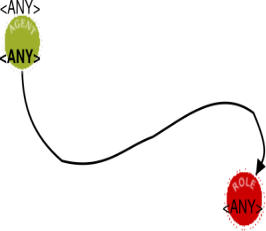
\includegraphics[width=.7\linewidth]{Chapiter3/img/L2}
	\linebreak  
	
	\hspace{2.5cm}  LHS 
\end{minipage}%
\begin{minipage}{.6\textwidth}
  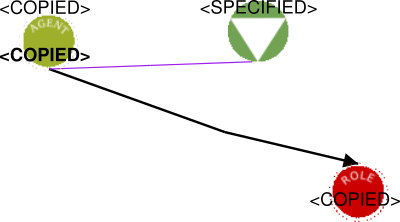
\includegraphics[width=.7\linewidth]{Chapiter3/img/R2}
  \linebreak  

  \hspace{2.5cm}  RHS 
\end{minipage}
\caption{\label{fig:Generate for each agent raw material}Transform Agent to Raw-material} 
\end{figure}
\vspace{1cm}

%% ------------------------------------------------------------------------------------------------ order 7 
\paragraph{\emph{3)~Transform Link between Agent and Role into Operating Unit (order7) :} }
 
 
This rule (Figure \ref{fig:Operating Unit for every link capable of playing}) allow to transform , the relation capable of playing between an agent and role  into operating unit .
\vspace{1cm}
\begin{figure}[th]
\centering
\begin{minipage}{.6\textwidth} 
  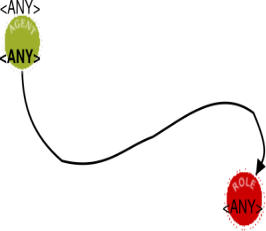
\includegraphics[width=.7\linewidth]{Chapiter3/img/L3}
  \linebreak  

\hspace{2.5cm}
  LHS 
  
\end{minipage}%
\begin{minipage}{.6\textwidth} 
  \includegraphics[width=.7\linewidth]{Chapiter3/img/R3}
  \linebreak  

\hspace{2.5cm}
  RHS  
\end{minipage}
\caption{\label{fig:Operating Unit for every link capable of playing}Transform CapableOf relation into operating unit} 
\end{figure}


%% ------------------------------------------------------------------------------------------------ order 9 
\paragraph{\emph{4)~Transform Goal to intermediate material (order9) :} }
 
 
Application of the rule illustrated in (Figure \ref{fig:Transform Goal to intermediate material}) Transform a goal in MaS into intermediate material in process system .

\vspace{1cm}
\begin{figure}[th]

\centering
\begin{minipage}{.6\textwidth}
 
  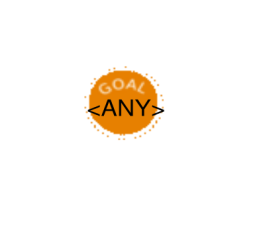
\includegraphics[width=.7\linewidth]{Chapiter3/img/L4}
  \linebreak

\hspace{2.5cm}  LHS
\end{minipage}%
\begin{minipage}{.6\textwidth}
 
  \includegraphics[width=.7\linewidth]{Chapiter3/img/R4}
\linebreak  

\hspace{2.5cm}  RHS 
\end{minipage}
\caption{\label{fig:Transform Goal to intermediate material}Transform Goal to intermediate material}
 
\end{figure}
 
%% ------------------------------------------------------------------------------------------------ order 10 
\paragraph{\emph{5)~Create the Product node (order10) :} }
 
 
Allow to Create the final material stat in the system like you notice the LHS is empty because this rule applied for one time , and this rule represented in 
(Figure \ref{fig:Create the final material} ) .


\vspace{1cm}
\begin{figure}[th]
\centering
\begin{minipage}{.6\textwidth}
 
  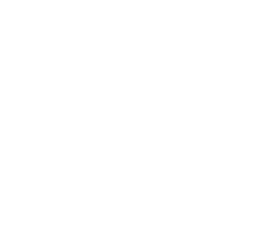
\includegraphics[width=.7\linewidth]{Chapiter3/img/L5}
  \linebreak

\hspace{2cm}  LHS
 
  
\end{minipage}%
\begin{minipage}{.6\textwidth}
 
  
\includegraphics[width=.7\linewidth]{Chapiter3/img/R5}
\linebreak  

\hspace{2.5cm}  RHS 
 
\end{minipage}
\caption{\label{fig:Create the final material}Create the final material}
 
\end{figure}
\vspace{1cm}

%% ------------------------------------------------------------------------------------------------ order  13
\paragraph{\emph{6)~Generate auxiliary part  (order 13) :} }
 
 
The Application of this rule generate the auxiliary part which is intermediate material consumed by operating unit , and the auxiliary part represent an agent capable to playing role in order to achieve a specific goal , you can see that from (Figure \ref{fig:Generate auxiliary part}) .
\vspace{1cm}
\begin{figure}[th]
\centering
\begin{minipage}{.6\textwidth}
 
  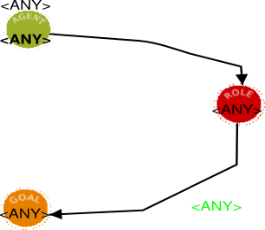
\includegraphics[width=.7\linewidth]{Chapiter3/img/L6}
  \linebreak

\hspace{2.5cm}  LHS
  
\end{minipage}%
\begin{minipage}{.6\textwidth}
 
  \includegraphics[width=.7\linewidth]{Chapiter3/img/R6}
\linebreak  

\hspace{2.5cm}  RHS  
\end{minipage}
\caption{\label{fig:Generate auxiliary part} Generate auxiliary part}
 
\end{figure}
\vspace{1cm}




%% ------------------------------------------------------------------------------------------------ order  15
\paragraph{\emph{7)~Create Operating unit between  goal material  and the product (order 15) :} }
 
 
The rule in (Figure \ref{fig:Create Operating unit between  goal and OAF}) 
it is to Create an operating unit  between the final material and the goals material .
  
\vspace{1cm}
\begin{figure}[th]
\centering
\begin{minipage}{.6\textwidth}
 
  \includegraphics[width=.7\linewidth]{Chapiter3/img/L7}
\linebreak  

\hspace{2.5cm}  LHS 
 
  
\end{minipage}%
\begin{minipage}{.6\textwidth}
 
  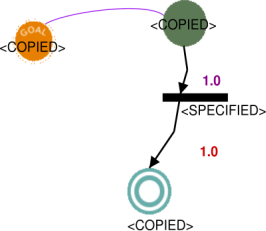
\includegraphics[width=.7\linewidth]{Chapiter3/img/R7}
\linebreak  

\hspace{2.5cm}  RHS 
\end{minipage}
\caption{\label{fig:Create Operating unit between  goal and OAF}Create Operating unit between  goal and OAF}
 
\end{figure}
\vspace{1cm}




%% ------------------------------------------------------------------------------------------------ order  19
\paragraph{\emph{8)~Create link between auxiliary part and  goal material  (order 19) :} }
 
 
The rule in (Figure \ref{fig:link between auxiliary part and goal})  describe 
how to link the auxiliary part with right goal .  
\vspace{1cm}
\begin{figure}[th]
\centering
\begin{minipage}{.6\textwidth}
 
  \includegraphics[width=.7\linewidth]{Chapiter3/img/L8}
  \linebreak

\hspace{2.5cm}  LHS
 
  
\end{minipage}%
\begin{minipage}{.6\textwidth}
 
  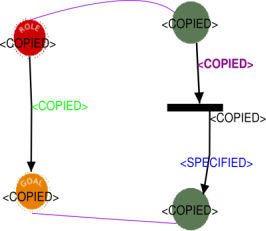
\includegraphics[width=.7\linewidth]{Chapiter3/img/R8}
\linebreak  

\hspace{2.5cm}  RHS 
 
\end{minipage}
\caption{\label{fig:link between auxiliary part and goal}link between auxiliary part and goal}
 
\end{figure}

\vspace{1cm}
%% ------------------------------------------------------------------------------------------------ order  20
\paragraph{\emph{9)~Create link to consume the raw material by operating unit  (order 20) :} }
 
 
This Figure \ref{fig:consume the raw material by operating unit}  illustrate  this rule , and it about how to create an arc between 
the raw material was generated from an agent and the operating unit .

 
\vspace{1cm}
\begin{figure}[th]
\centering
\begin{minipage}{.6\textwidth}
 
  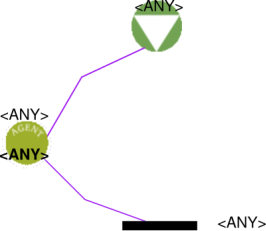
\includegraphics[width=.7\linewidth]{Chapiter3/img/L9}
  \linebreak

\hspace{2.5cm}  LHS
 
  
\end{minipage}%
\begin{minipage}{.6\textwidth}
 
  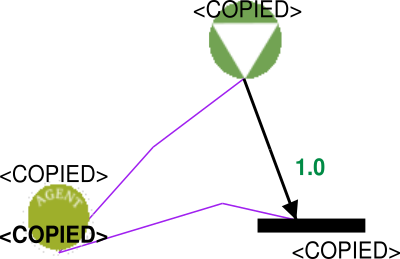
\includegraphics[width=.7\linewidth]{Chapiter3/img/R9}
\linebreak  

\hspace{2.5cm}  RHS 
 
\end{minipage}
\caption{\label{fig:consume the raw material by operating unit} consume the raw material by operating unit}
 
\end{figure}
\vspace{1cm}

after that you notice some key word in  :
\begin{itemize}
\item Left hand side
	\begin{enumerate}
	\item ANY : its attribue in the node and the engine will select every node with ANY attribute value
	\end{enumerate}
\item  Right hand side
	\begin{enumerate}
	\item COPIED : copie the attribue value from the node with same GGLabel in LHS
	\item SPECIFIED : specified the attribue value manualy or by code 
	\end{enumerate}
\end{itemize}
 
you know  every rule have condition , the figures illustrate 3 condition for 3 rule 

 
\paragraph{\emph{1)~Condition for the rule   Assign Role to Agent  :  } } 
 
That condition test if there node agent , role visited before 
In order not to fall in infinity loop , figure \ref{fig:Create link between Agent and Role} represent the rule .
 
\begin{figure}[th]
	\centering
 	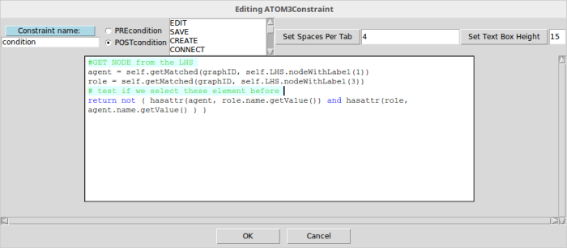
\includegraphics[scale=0.8]{Chapiter3/img/condrule1}
	\caption{\label{fig:Condition link agent with role}Condition link agent with role  }
\end{figure} 
\pagebreak 
\paragraph{\emph{2)~Condition for Create Final Stat : } } 
That condition test if this attribute Final stat equal zero 
, in other word we did not visite this rule before , the rule in figure\ref{fig:Create the final material} .
 
 
\begin{figure}[th]
	\centering
 	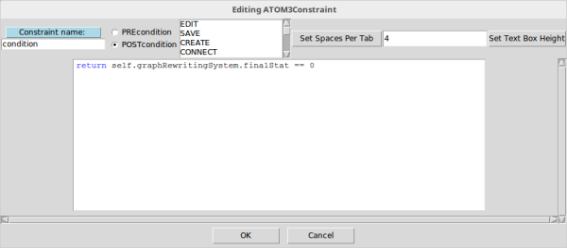
\includegraphics[scale=0.8]{Chapiter3/img/condfinal}
	\caption{\label{fig:Condition of generate final stat } Condition of generate final stat }
\end{figure} 
 

\paragraph{\emph{3)~Condition of rule link between AUX part and Material Goal } : }
  
 
Test if we did not visited before  and the name of Auxiliary Part end with goal name to link it with the right goal material , the rule in figure \ref{fig:link between auxiliary part and goal}  .
 
 
 
\begin{figure}[th]
	\centering
 	\includegraphics[scale=0.8]{Chapiter3/img/condaux}
	\caption{\label{fig:Condition of Auxiliary part}Condition of Auxiliary part  }
\end{figure} 





\pagebreak
\subsection{ Examples }

\subsubsection{ Simple multi Agent System }
This example represents a very simple system composed of  two agent and 3 capabilities , 2 role and 2 goals  .
 Figure \ref{fig:Example 1 Multi Agent System } illustrates this example :
\begin{figure}[th]
	\centering
 	\includegraphics[scale=0.8]{Chapiter3/img/ex1omacs}
	\caption{\label{fig:Example 1 Multi Agent System }Example 1 Multi Agent System}
\end{figure} 
 
The purpose of this example is to demonstrate the transformation of multi agent system in OMACS into pns model

Figure \ref{fig:Multi Agent System After transformation } shows the transformation result.
It is clear that the resulting contain set of material and operating unit
 
\begin{itemize}
\item the raw material A1 , A2 represent the agent from last model
\item the operating unit A1 R1 represent the relation between an A1 and R1 
in Mas before the transformation its the same for other entities like this one
\item the operating unit and material named A2 R2 G2 represent agent A2 Playing R2 in order to achieve G2 , it is the same for other entities  

\item the operating unit and material named A2 R2 G2 represent agent A2 Playing R2 in order to achieve G2 


\item the operating unit and material named A1 R1 G2 represent agent A1 Playing R1 in order to achieve G2  and G2 , any agent in this is capable to play R1 can reach G1 and G2
 

\end{itemize}
  


\begin{figure}[th]
	\centering
 	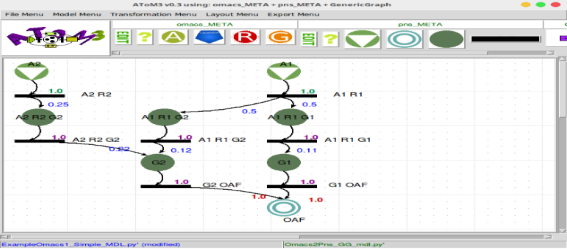
\includegraphics[scale=0.8]{Chapiter3/img/ex1pns}
	\caption{\label{fig:Multi Agent System After transformation }Multi Agent System After transformation}
\end{figure}  
\subsubsection{ Complex multi Agent System }
This example represents a complex system composed of  3 agent and 4 capabilities , 2 role and 4 goals  . Figure \ref{fig:Example 1 Multi Agent System } illustrates this example ,
 


\begin{figure}[th]
	\centering
 	\includegraphics[scale=0.8]{Chapiter3/img/article}
	\caption{\label{fig:Complex Multi Agent System}Complex Multi Agent System}
\end{figure} 

\begin{itemize}
	\item every agent possesses set of capabilites for example A1 possese all capabilies in the system
	\item Role require list of capabilies every agent has the same capabilies or more , so he can play this role
	\item Role R1 , R2 achieve all goal in the system
	\item the Agent A1 all capabilites in the system so we can say , A1 capable of playing R1 and R2
	\item Agent A1 capable of playing all roles in this system , so he can achieve all goal in the system
\end{itemize}

after the Transformation of Multi agent system from OMACS frame into PNS framework we get this model in figure \ref{fig:Complex Multi Agent System After transforamtion} 
and next table represent the value of this model 

 % Please add the following required packages to your document preamble:
% \usepackage{booktabs}
\begin{table}[]
\centering
\begin{tabular}{@{}ccc@{}}
\toprule
\textbf{Operating Unit} & \textbf{Input Material} & \textbf{Output Material}                                                                              \\ \midrule
G1OAF                   & G1(1)                   & OAF (1)                                                                                               \\
G2OAF                   & G2(1)                   & OAF(1)                                                                                                \\
G3OAF                   & G3(1)                   & OAF(1)                                                                                                \\
G4OAF                   & G4(1)                   & OAF(1)                                                                                                \\ \midrule
A1R1G1                  & A1R1G1(0.433)           & G1(0.2)                                                                                               \\
A1R1G2                  & A1R1G2(0.433)           & G2(0.4)                                                                                               \\
A1R1G3                  & A1R1G3(0.433)           & G3(0.6)                                                                                               \\
A1R1G4                  & A1R1G4(0.433)           & G4(0.8)                                                                                               \\
A1R2G1                  & A1R2G1(0.433)           & G1(1.0)                                                                                               \\
A1R2G2                  & A1R2G2(0.433)           & G2(0.7)                                                                                               \\
A1R2G3                  & A1R2G3(0.433)           & G3(0.4)                                                                                               \\
A1R2G4                  & A1R2G4(0.433)           & G4(0.1)                                                                                               \\
A2R2G1                  & A2R2G1(0.633)           & G1(1.0)                                                                                               \\
A2R2G2                  & A2R2G2(0.633)           & G2(0.7)                                                                                               \\
A2R2G3                  & A2R2G3(0.633)           & G3(0.4)                                                                                               \\
A2R2G4                  & A2R2G4(0.633)           & G4(0.1)                                                                                               \\
A3R2G1                  & A3R2G1(0.5)             & G1(1.0)                                                                                               \\
A3R2G2                  & A3R2G2(0.5)             & G2(0.7)                                                                                               \\
A3R2G3                  & A3R2G3(0.5)             & G3(0.4)                                                                                               \\
A3R2G4                  & A3R2G4(0.5)             & G4(0.1)                                                                                               \\ \midrule
A1R1                    & A1                      & \begin{tabular}[c]{@{}c@{}}A1R1G1(0.433) ,A1R1G2(0.433) \\ ,A1R1G3(0.433) ,A1R1G4(0.433)\end{tabular} \\ \midrule
A1R2                    & A1                      & \begin{tabular}[c]{@{}c@{}}A1R2G1(0.433) ,A1R2G2(0.433) ,\\ A1R2G3(0.433) ,A1R2G4(0.433)\end{tabular} \\ \midrule
A2R2                    & A2                      & \begin{tabular}[c]{@{}c@{}}A2R2G1(0.633) ,A2R2G2(0.633) ,\\ A2R2G3(0.633) ,A2R2G4(0.633)\end{tabular} \\ \midrule
A3R2                    & A3                      & \begin{tabular}[c]{@{}c@{}}A3R2G1(0.5) ,A3R2G2(0.5) ,\\ A3R2G3(0.5) ,A3R2G4(0.5)\end{tabular}         \\ \bottomrule
\end{tabular}

\caption{Value of PNS Model}
\label{Value of PNS Model}
\end{table}


% Add table HEre
 \begin{landscape}
\begin{figure}[th]
	\centering 
 	\includegraphics[scale=1.3]{Chapiter3/img/articlePNS2}
	\caption{\label{fig:Complex Multi Agent System After transforamtion}Complex Multi Agent System After transforamtion}
\end{figure} 
 
 \end{landscape}


% now we have the MaS in PNS Form 
% and there Tools called PGraphStudio
%
%
\section{Transformation Approach ( PNS into XML file ) }
In Section \ref{sec:OMACS into PNS} we presented our transformation approach That allows 
to transform the OMACS to PNS .

The purpose of this transformation is the Optimization and for this we
Proposed Another processing approach That transforms PNS to XML 
files to analysis for a optimization tool 
\subsection{ Graph Grammar }
 this grammar is Composed of three parts: 
\begin{itemize}
\item \textbf{Initial Action : } This portion of our grammar is used to initialize all
Global variables used. They are used to meet various needs.  in Figure \ref{fig:Code Initial Action} 

\end{itemize}

\begin{figure}[th]
	\centering  %[scale=1.2]
 	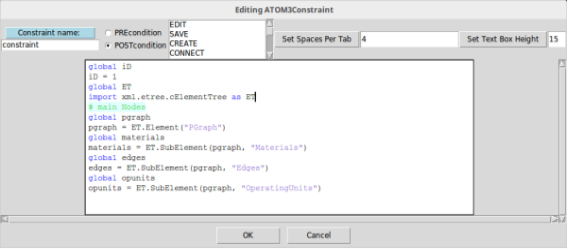
\includegraphics[scale=0.8]{Chapiter3/img/InitAct}
	\caption{\label{fig:Code Initial Action}Code Initial Action}
\end{figure} 

\begin{itemize}
\item \textbf{Final Action : } Final Action Allows Completing the .xml file by the tags
XML Completing the after-processing of all PNS nodes and save the page name. in figure \ref{fig:Code Final Action} 
   
\end{itemize}

\begin{figure}[th]
	\centering  %[scale=1.2]
 	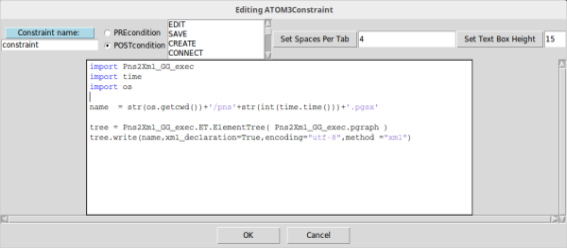
\includegraphics[scale=0.8]{Chapiter3/img/FinAct}
	\caption{\label{fig:Code Final Action}Code Final Action}
\end{figure} 
\pagebreak
\begin{itemize}
\item \textbf{ Set of Rules : } 
 
Our grammar graphs Consists of ten rules. Each
rule is Characterized by a name and an execution priority. 

\end{itemize}
 We quote here The Most major rules: 
\paragraph{\emph{1)~Transform RawMaterial into XML code :} }
This rule (Figure \ref{fig:Raw Material into Xml}) to priority equal to "1", ie, 
it is the first rule applied on the Model . She transforms the place into a XML

\begin{figure}[th]
\centering
\begin{minipage}{.6\textwidth}
 
  \includegraphics[width=.7\linewidth]{Chapiter3/img/xL1}
  \linebreak

\hspace{2.5cm}  LHS
 
  
\end{minipage}%
\begin{minipage}{.6\textwidth}
 
  
\includegraphics[width=.7\linewidth]{Chapiter3/img/xR1}
\linebreak  

\hspace{2.5cm}  RHS 
 
\end{minipage}
\caption{\label{fig:Raw Material into Xml}Raw Material into Xml} 

\end{figure} 

\pagebreak
\paragraph{\emph{ a )~Condition for rule \ref{fig:Raw Material into Xml} } } For the application of this rule, it must be verified that the partition To be transformed is not treated before

\begin{figure}[th]
	\centering  %[scale=1.2]
 	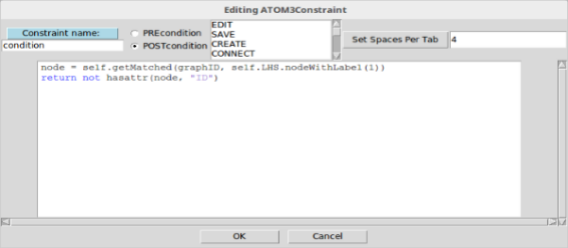
\includegraphics[scale=1.1]{Chapiter3/img/xcond1}
	\caption{\label{fig:condition of Raw Material for Transfromation}condition of Raw Material for Transfromation}
\end{figure}
\paragraph{\emph{ b )~Action for rule \ref{fig:Raw Material into Xml} } }  Once the rule is applied, it Action Allows to create a code INSTEAD XML and mark the object to the left side to processed.  
 
\begin{figure}[th]
	\centering  %[scale=1.2]
 	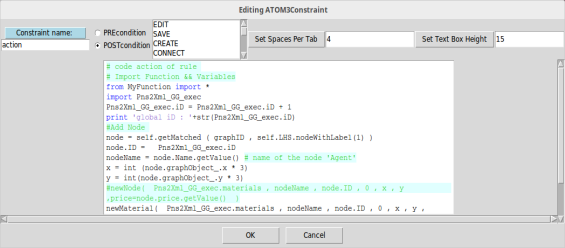
\includegraphics[scale=0.66]{Chapiter3/img/xact1}
	\caption{\label{fig:Action of Raw Material for Transfromation}Action of Raw Material for Transfromation}
\end{figure} 
\vspace{1cm}
like you see in the first line i import MyFunction is external file , Python code 
to be easy to manipulate  and this is the function to add new material ( raw , intermadiate , final)
and for the operating unit is the similair function
 
\vspace{1cm}
\begin{lstlisting}[language=Python, caption=Python Function Material]
def newMaterial(  parent=None , name= "None" , ID="0" , Type= "None" , xN ='-1', yN ='-1' ,price='-1' ,reqF = 0  ,maxF =999999 ):
	#Create new Node has the Material Name ...and add it into the parent node
	node = ET.SubElement(parent, "Material",ID=str(ID),Name=name,Type=str(Type))
    print 'add Cords into node		-NewNode-'
	#Create Corde for the node material
	cords = ET.SubElement(node, "Coords")
	ET.SubElement(cords, "X").text = str( xN )
	ET.SubElement(cords, "Y").text = str( yN )
	#Test if the patameter is not null or empty
	if price != '-1' or  reqF != 0  or maxF !=999999 : 
		ParameterList = ET.SubElement(node, "ParameterList")
		ET.SubElement(ParameterList, "Parameter",Name="price",Value=str( price) )
		if reqF == 0 : reqF = '-1'
		ET.SubElement(ParameterList, "Parameter",Name="reqflow",Value= str(reqF) )
		if maxF == 999999 : maxF = '-1'
		ET.SubElement(ParameterList, "Parameter",Name="maxflow",Value=str(maxF) )

	#Create Label for the MaterialNode
	label = ET.SubElement(node, "Label",Text = str(name))
	offset = ET.SubElement(label,  "Offset")
	ET.SubElement(offset, "X").text =   str(5)
	ET.SubElement(offset, "Y").text =   str(0)
	
	return node
\end{lstlisting}

\paragraph{\emph{2)~Transform Edge between two entitie into XML code :} } in this transformation 
we want to create link between nodes Material and Operating unit 
and we have  4 type of Edges : 
\begin{itemize}
	\item Edges from raw material into Operating unit
	\item Edges from intermediate material into Operating unit
	
	\item Edges from  Operating unit into final material
	\item Edges from  Operating unit into intermadiate material 
\end{itemize}
and the figure \ref{fig:edgotoraw} represent the first Edge type 

\begin{figure}[th]
\centering
\begin{minipage}{.6\textwidth}
 
  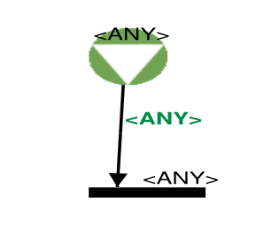
\includegraphics[width=.7\linewidth]{Chapiter3/img/xL2}
  \linebreak

\hspace{2.5cm}  LHS
 
  
\end{minipage}%
\begin{minipage}{.6\textwidth}
 
  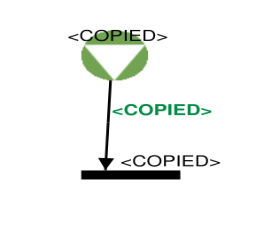
\includegraphics[width=.7\linewidth]{Chapiter3/img/xR2}
\linebreak  

\hspace{2.5cm}  RHS 
 
\end{minipage}
\caption{\label{fig:edgotoraw}Edges from Raw Material into Operating unit to xml code} 

\end{figure} 
 
\pagebreak
\paragraph{\emph{ a )~Condition for rule \ref{fig:edgotoraw} } } it is the same with figure \ref{fig:condition of Raw Material for Transfromation} but here we select the edges

\vspace{1cm} 
\begin{figure}[th]
	\centering  %[scale=1.2]
 	\includegraphics[scale=0.8]{Chapiter3/img/xcond2}
	\caption{\label{fig:Condition2)}Condition of Edges ( RawMaterial to Operating unit)}
 \end{figure} 
\vspace{1cm}
\paragraph{\emph{ b )~Action for rule \ref{fig:edgotoraw} } }  we add this action to  Transform the Edges between Any Material and Any Operating unit into xml file  , or to export the entitie from Graphical presentation 
into Xml Code  
\pagebreak 


\begin{figure}[th]
	\centering  %[scale=1.2]
 	\includegraphics[scale=0.8]{Chapiter3/img/xact2}
	\caption{\label{fig:action2)}Action of Edges ( RawMaterial to Operating unit)}
\end{figure}  

and this code represent a Function to add new Edges into the Tree code 
to export the tree later 

\begin{lstlisting}[language=Python, caption=Python Function new Edges]
def newEdges(  parent  , name  , ID    , xN  , yN    ,beginID   , endID    ):
	#Create new Node and add it into parent Node	
	node = ET.SubElement(parent, "Edge",ID=str(ID),BeginID=str(beginID),EndID=str(endID),Rate=str(name),Title=str(name) , ArrowOnCenter="true" , ArrowPosition="50")  
	
	#Create Corde for the node Edges
	cords = ET.SubElement(node, "Coords")
	ET.SubElement(cords, "X").text = str( xN )
	ET.SubElement(cords, "Y").text = str( yN )
		 		 		  
	#Create Label for the Edges
	label = ET.SubElement(node, "Label",Text = str(name))
	offset = ET.SubElement(label,  "Offset")
	ET.SubElement(offset, "X").text =   str(5)
	ET.SubElement(offset, "Y").text =   str(0)
 
	return node 
\end{lstlisting}

% UPDATE 13.47
